As the back end is responsible for performing the image synthesis it contains the majority of the code that requires disscussion.

\subsection{Photon Emission(3 pages)}
Once the scene data has been created it is passed to the back-end, the first step that is performed is photon gathering,
in this stage photons are emmited from all light sources in the scene and are stored in one of the photon maps for use
in the raytracing stage of the algoithm, as discussed in the design chapter the emission of the photons is performed in
parralell using pthreads, each thread is started with a data structure that contains the scene into which the photons
are being emmited from and the number of photons the thread is responsible for storing in the photon map, for each photon
that is to be stored we write to a queue that is read by the main thread. along with the photon traced a summary of the
path of the photon is written in the queue. Once all of the photons have been emitted a flag is set to inform that the
thread is finished, this is sent along the same channel as the photons. The number of photons that are emmited is determined
by the power of each of the lights, as a result lights with higher power will have more photons emitted for that light as
we need to be able to calculate the contribution from these light sources with more accuracy than lights with lower power
as they contribure more to the illuminaion of the scene.

\subsection{Photon Generation}
In order to emit photons into the scene we need a method of creating photons, this is implemented in the light defintion,
each light object has a associated function that will produce a random photon from the light that is consitent with the
type of light, for instance a point light will generate a photon with origin exactlu at the origin of the light source and
in a random direction, an area light produces a photon with origin on the area of the light with direction taken from a
cosine weighted hemisphere distribution in the direction of the normal of the light. Each photon that is emitted from the
light sources begin with the full power of the light source, this will be scaled by the number of emitted photons after
all photons have been gathered.

As discussed in \todo{Jensen Citation} at each interaction with a non-specular surface the power of the reflected photon
needs to be scaled by the reflectance of the surface, this would insert many low power into the photon map, he suggests
using monte carlo sampling and russian roulette to create a photon with probablilty proportional to the reflectance
of the surface.

Storing the photons is performed at each interaction with a non specular surface, the reason for not storing at specular
surface is that specular BRDFs contain the dirac delta function as a result the photon map cannot be used to evaluate the
radiance at this point, we use traditional raytracing to perform the radiance at specular surfaces.

\subsection{Volume Photon Map}
When tracing the photons through the scene and it intersects with a participating media we begin by transmitting the
photon into the media based on the surface properties of the media, after this we iterativly scatter the photon in the
media storing the photon at each of the points of scattering, the scattering is determined by the scattering and
absorbtion coefficients of the media, the media has a component for each of the colour components, when moving through
the volume the power of the photon is reduced much like the reduction for reflections at surfaces, like surfaces this
would end with many low power photons in the map instead we perform importance sampling by modifiing the distance that
the photon moves through the media inbetween interactions with the media, equation \todo{Add the fucntion and a citation}
is used for the importance sampling.

\missingfigure{Volume Photon Map}

\missingfigure{Surface Photon Map}

\begin{figure}
\begin{lstlisting}
struct thread_output_data
{
	char last      : 1;
	char diffuse   : 1;
	char specular  : 1;
	char light     : 5;
	union
	{
		photon_t photon;
		int      emitted;
	};
};
\end{lstlisting}
\caption{Output of photon emittion threads}
\end{figure}

\subsubsection{Algorithmic Overview}

\begin{algorithm}[h!]
	\KwData{Scene Description}
	\KwResult{Photon paps for input scene}
	\For{each light in scene}
	{
		TracePhoton(photon);
	}
	\caption{Photon mapping algothm}
\end{algorithm}

\begin{algorithm}[h!]
	\KwData{Scene Description, Photon}
	\KwResult{Photon added to photon map}
	\eIf{photon intersects scene}
	{
	
	}
	{
		Discard photon;
	}
\caption{TracePhoton}
\end{algorithm}

\subsection{Photon Data Structure (0.5 page)}
As noted by Jensen \todo{cite} the need for a compact representation of the individual photons in the photon map is vital
as it is typical for their to be many thousands to millions of photons in order to perform accurate radiance estimates,
the initial implementation of the photon map included a naive implementation that used double width floating point values.
\todo{Analysis for speed}

\subsection{K-D Tree Balancing (1 page)}
When performing radiance estimations with the photon map we will be performing nearest neighbour searches on points within
the map, this requires the photon map to be arrainged in a manner such that this search can be performed efficiently.
In order to do this we store the photon map in a left-balanced k-d tree. A left balanced tree is a tree structure where
at each level of the tree the depth of the children differs by at most one, \todo{finish the explination of the LEFT balanced tree}
this allows us to store the photon map in an array with the location of the children in the photon map known implicitly,
for a photon in position $i$ the children of the photon can be found at the $(2i + 1)^{th}$ and $(2i + 2)^{th}$
location for the left and right tree respectivly.

\todo{Add the median of median algorithm here}

\begin{figure}
\centering
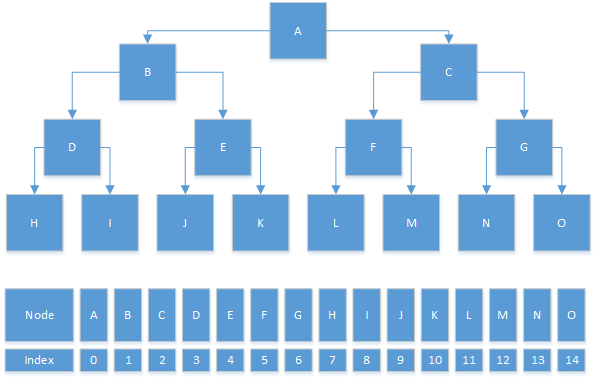
\includegraphics[scale=0.75]{./implementation/left-balanced-tree.png}
\caption{Left balanced tree and its memory layout}
\end{figure}

\subsection{Selection Statistic}
During the balancing procedure we need to partition the tree such that half the elements are less than the median
this can be seen as finding the $i/2^{th}$ largest element in the list, this can be performed in linear time by using
the median of medians algorithm \todo{cite}. Below is a comparison for the runnning time of the balancing procedure for
the nieve selection algorithm and the median of medians algorithm. As we are left-balancing the tree we also cannot
just take the median of the data, we must adjust the median such that the left half of the tree will fill before the right.

\missingfigure{times for median of median compared}

\subsection{Photon Termination}
During the photon tracing stage at each of the intersections that are found we must make a choice whether to refect absorb or transmit
the photon, for purely specular materials the choice is simple, that is we will reflect the photon. For materials that are not purely
specular such as diffuse materials the choice is less clear, we must take into account the BDRF of the material.

\section{Raytracing (10 pages)}
\begin{algorithm}[H]
\For{each pixel in output image}
{
	send pixel x, y to thread queue;
}

finish\_count := 0;

\While{finish\_count != thread\_count}
{
	data := read from output queue

	\If{data == pixel\_data}
	{
		send pixel data back to front end
	}
	\Else
	{
		finish\_count := finish\_count + 1;
	}
}

\caption{Raytracing Algorithm}
\end{algorithm}

\subsection{Algorithmic Overview}

\subsection{Threading Model (0.5 pages)}
As noted in the design section of this document raytracing related rendering methods are inherently easily parrelised as each
ray can be traced in its own thread, the method that the system uses to distribute the work that is needed to be done is
based on a producer consumer model whereby the work is fed into a queue of work items that can be read by any of the worker
threads, in order to perform this a queue implementation was needed, this can be found in the \texttt{queue.c} source file,
this queue is thread-safe and as such is suitable for this use case. When working with multiple threads it is important
to prevent as much global state as possible, within the system this is no different and as a rule global variables are not used
with the exception of the configuration structure, this is due to the fact that after the initial setup of the scene the data
during the start of the programs execution no data within the structure is permitted to be modified and as such can be read
safety from any thread. In order to inform each thread that all pixels have been processed a dummy input is sent to each of the
threads, on reading this input the thread will return.

\missingfigure{Threading Model}

The choice of mulitthreading library that I have used is pthreads. Posix threads are a definition
of a threading model that allows C programs to be run on muliple threads, pthreads are defined for unix like systems so
linux and mac os are supported so partially fulfills requirement \todo{add requerement refs}: as windows does not have native
support for pthreads, there is however an implementation that uses native Windows threads to present the types and functions defined
by pthreads. As I am using C11 it could be possible to use the threading functionallity that is defined in the standard,
unfortunatally the support for this feature is largly unsupported (as of \today).

\subsection{Pixel Sampling}
As the raytracer is performing distribution raytracing each thread will perform multiple raytracing operations for each pixel
that it processes each sample per pixel is offset inside the pixel to perform antialiasing, this reduces the sharp edges that
can be seen in images. In order to improve the appearence of the image we also perform jittering on the samples this reduces
certain artifacts such as banding. \todo{Make sure the banding comment is correct and if so find a reference for it}

\missingfigure{anti-aliasing}

\subsection{Intersection Storage}
When raytracing the scene the intersection point of the ray needs to be calculated and stored, this will include data that
is specific to an objects intersection, for example an intersection with a triangle mesh will need to record the trangle
that was intersected and as a result will need to record the barycentric coordinate at the point of intersection.

\subsection{Object System}
In order to meet requirement \todo(find requirement to ref) the system needs to be able support arbitrary objects descriptions
that can be traced in the scene, this is implementatied as a structure that contains function pointers that perform functions
that must be supported by all raytracable objects and the data related to the individual object.

\begin{description}
\item[normal] returns the normal at a point of intersection.
\item[bounds] return the bounds for the object.
\item[texture] return the texture coordinates at a point of intersection
\item[intersection] returns if a ray intersects a given object.
\end{description}

By encapsulating the data and the functions performed by the object it is possible to create algorithms on objects in the
abstract such that the details of the object can be ignored, for instance calculating a reflected ray at a point if intersection
is a function of only the surface normal at that point, wheither it is a triangle mesh or sphere the same ray will be calculated.

\subsubsection{Texture Mapping}
Performing texture mapping requires the ability to query the texture coordinates at a point of intersection, for mesh objects this
will interpolate the barycentric coordinates for the triangle of intersection, spheres use a spherical mapping that uses the
spherical coordinates to generate u,v values.

\subsubsection{Mesh}
\subsubsection{Sphere}
\subsubsection{Participating Media}

\subsection{K-D Tree Construction}
In order to satisy requirement TODO:Add the requirement bruteforce methods for raytracing are not acceptable, in order to reduce
to number of intersection tests that are performed I have decided to use the kdtree for the accelleration structure. The
construction of the kdtree is performed during the initialiseation of the triangle meshes as it is a static data structure, due
to it being a static data structure their is an advantage to performing more extensive computation in the construction in
order to create a higher quality of kdtree. TODO:Add sah and analysis.

\subsection{Intersection Tests (0.5 pages)}
Intersection tests are another vital part of any raytracer. a number of intersection tests are needed, I will not include
an extensive treatment of the intersection tests mearly a listing of the most notable used.

\begin{description}
\item[Triangle] Moller-Trumbore intersection test \cite{MolTru97}
\item[AABB]
\item[kD-tree] As described in TODO:
\end{description}

\subsection{Photon Mapping}
For each of the intersection points that are found as a result of the raytracing algorithm we must calculate the global
illumination at the point, this is performed with the photon maps that are associated with the scene.

\subsection{Nearest Neighbour search}
\todo{Find the correct location for this}
By far the most expensive operation in the photon mapping algorithm is the nearest neghbour search as we perform
many more of these operations per pixel, for radiance estimates that contain tens, hundreeds or thousands of photons
efficiently finding the $n$ closest photons is important.

\missingfigure{Nearest neighbour search}

\subsection{Sampling Strategy}
Many times within the code there is a need to sample from different distributions such as sampling from a hemisphere
of directions around a normal, the need for this can be seen from the definition of the radiance estimate given in
the desctription of the photon mapping algorithm as we will be evaluating the integral with monte carlo methods.

\subsection{Shading}
The intersection point of the primary ray is used as the point where we will evaluate the radiance for that will determin
the colour of the pixel, this is done by combining the result of direct lighting, indirect lighting, castics and if present
scattering and attenuation due to participating media, this is commonly expressed as a sum of integrals that sum to a solution
to the rendering equation, equation \todo{Add the equation} shows this.

\subsubsection{Direct Illumination}
Direct illumination can be calculated direclty by calculating the radiance incident to the intersection point for each of the
lights in the scene.

\missingfigure{Direct Illumination}

\subsubsection{Caustic Contribution}
Caustic illumintation indirect illumitionan from photons that take purly specular paths prior to being stored at a non-specular
surface.

\subsubsection{Multiple diffuse bounves and final gathering}

While it is possible to estimate the contribition to the radiance at an intersection point directly from the photon map this
approach can cause visual artifacts due to variance in the estimate in order to reduce these artifacts we perfom a final gather
stage at the point of intersect that produces a diffuse ray that is traced into the scene until a non-specular object is intesected,
we then perform the radiance at this point and use this information to estimate the radiance incident at the original point of intersection.
In order for the final gather to produce a correct estimate of the radiance we need to perform this stage multiple times per pixel, as we
are performing distributed raytracing this is a trivial addition. When calcualting the radiance for the final gather it has been shown \todo{cite}
that if the distance of the final gather point is lower than some threshold perfoming an additional diffuse bounce reduces errors at geometry
such as sharp corners where the radiance estimate can be inaccurate due to accounting for photons not truly at the surface.

\begin{figure}
\centering
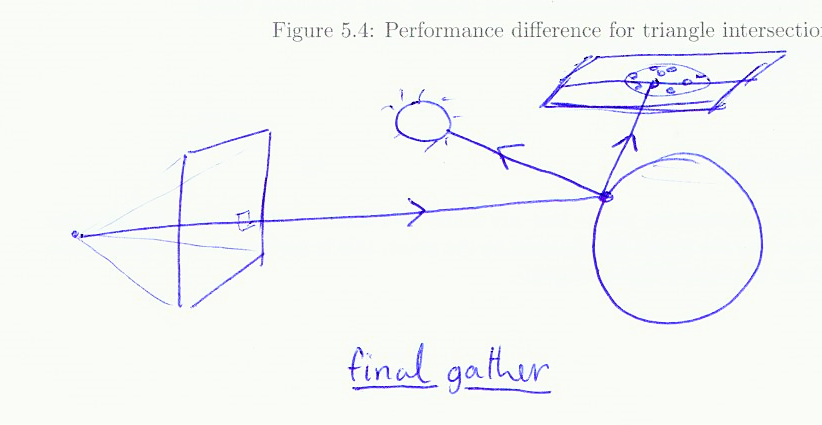
\includegraphics[width=\textwidth]{./images/final_gather.png}
\label{fig:final_gather}
\caption{Final Gather}
\end{figure}

\subsection{Volume Contribution}
In the case of a ray that intersects a participating media before intersecting a surface we need to calculate three components to
the radiance along the path of the ray in the medium, these are single scattering direct illumination, multiple scattering (in-scattering)
and attenuation (out-scattering)

\subsubsection{Attenuation}
As a ray travels through a medium the radiance can be reduced due to out-scattering and absortion, this can be calculated by evaluating
the integral given in equation \todo{Add the equation}, as we are only considering homogeneous participating media this can be
simplified as the properties being integrated are constant and a closed form solution is possible.

\missingfigure{Attenuation Equation}

\subsubsection{Direct Illumination}
\subsubsection{Muliple Scattering}

